\documentclass[english,floatsintext,man]{apa6}

\usepackage{amssymb,amsmath}
\usepackage{ifxetex,ifluatex}
\usepackage{fixltx2e} % provides \textsubscript
\ifnum 0\ifxetex 1\fi\ifluatex 1\fi=0 % if pdftex
  \usepackage[T1]{fontenc}
  \usepackage[utf8]{inputenc}
\else % if luatex or xelatex
  \ifxetex
    \usepackage{mathspec}
    \usepackage{xltxtra,xunicode}
  \else
    \usepackage{fontspec}
  \fi
  \defaultfontfeatures{Mapping=tex-text,Scale=MatchLowercase}
  \newcommand{\euro}{€}
\fi
% use upquote if available, for straight quotes in verbatim environments
\IfFileExists{upquote.sty}{\usepackage{upquote}}{}
% use microtype if available
\IfFileExists{microtype.sty}{\usepackage{microtype}}{}

% Table formatting
\usepackage{longtable, booktabs}
\usepackage{lscape}
% \usepackage[counterclockwise]{rotating}   % Landscape page setup for large tables
\usepackage{multirow}		% Table styling
\usepackage{tabularx}		% Control Column width
\usepackage[flushleft]{threeparttable}	% Allows for three part tables with a specified notes section
\usepackage{threeparttablex}            % Lets threeparttable work with longtable

% Create new environments so endfloat can handle them
% \newenvironment{ltable}
%   {\begin{landscape}\begin{center}\begin{threeparttable}}
%   {\end{threeparttable}\end{center}\end{landscape}}

\newenvironment{lltable}
  {\begin{landscape}\begin{center}\begin{ThreePartTable}}
  {\end{ThreePartTable}\end{center}\end{landscape}}




% The following enables adjusting longtable caption width to table width
% Solution found at http://golatex.de/longtable-mit-caption-so-breit-wie-die-tabelle-t15767.html
\makeatletter
\newcommand\LastLTentrywidth{1em}
\newlength\longtablewidth
\setlength{\longtablewidth}{1in}
\newcommand\getlongtablewidth{%
 \begingroup
  \ifcsname LT@\roman{LT@tables}\endcsname
  \global\longtablewidth=0pt
  \renewcommand\LT@entry[2]{\global\advance\longtablewidth by ##2\relax\gdef\LastLTentrywidth{##2}}%
  \@nameuse{LT@\roman{LT@tables}}%
  \fi
\endgroup}


\ifxetex
  \usepackage[setpagesize=false, % page size defined by xetex
              unicode=false, % unicode breaks when used with xetex
              xetex]{hyperref}
\else
  \usepackage[unicode=true]{hyperref}
\fi
\hypersetup{breaklinks=true,
            pdfauthor={},
            pdftitle={Performance of students in Math and Porgugese},
            colorlinks=true,
            citecolor=blue,
            urlcolor=blue,
            linkcolor=black,
            pdfborder={0 0 0}}
\urlstyle{same}  % don't use monospace font for urls

\setlength{\parindent}{0pt}
%\setlength{\parskip}{0pt plus 0pt minus 0pt}

\setlength{\emergencystretch}{3em}  % prevent overfull lines

\ifxetex
  \usepackage{polyglossia}
  \setmainlanguage{}
\else
  \usepackage[english]{babel}
\fi

% Manuscript styling
\captionsetup{font=singlespacing,justification=justified}
\usepackage{csquotes}
\usepackage{upgreek}



\usepackage{tikz} % Variable definition to generate author note

% fix for \tightlist problem in pandoc 1.14
\providecommand{\tightlist}{%
  \setlength{\itemsep}{0pt}\setlength{\parskip}{0pt}}

% Essential manuscript parts
  \title{Performance of students in Math and Porgugese}

  \shorttitle{education}


  \author{Nathaniel Phillips\textsuperscript{1}}

  \def\affdep{{""}}%
  \def\affcity{{""}}%

  \affiliation{
    \vspace{0.5cm}
          \textsuperscript{1} University of Basel  }

 % If no author_note is defined give only author information if available
      \newcounter{author}
                              \authornote{
            Correspondence concerning this article should be addressed to Nathaniel Phillips, Missionsstrasse 62A 4053 Basel Switzerland. E-mail: \href{mailto:nathaniel.phillips@unibas.ch}{\nolinkurl{nathaniel.phillips@unibas.ch}}
          }
                    
  \note{These data come from the UCI Machine Learning database at
\url{http://archive.ics.uci.edu/ml/datasets/Student+Performance\#}}

  \abstract{This data approach student achievement in secondary education of two
Portuguese schools. The data attributes include student grades,
demographic, social and school related features) and it was collected by
using school reports and questionnaires. Two datasets are provided
regarding the performance in two distinct subjects: Mathematics (mat)
and Portuguese language (por).}
  \keywords{apa, R, markdown \\

    \indent Word count: X
  }





\usepackage{amsthm}
\newtheorem{theorem}{Theorem}
\newtheorem{lemma}{Lemma}
\theoremstyle{definition}
\newtheorem{definition}{Definition}
\newtheorem{corollary}{Corollary}
\newtheorem{proposition}{Proposition}
\theoremstyle{definition}
\newtheorem{example}{Example}
\theoremstyle{definition}
\newtheorem{exercise}{Exercise}
\theoremstyle{remark}
\newtheorem*{remark}{Remark}
\newtheorem*{solution}{Solution}
\begin{document}

\maketitle

\setcounter{secnumdepth}{0}



What is the relationship between student performance in language and
mathematics tasks? This is an important question that has been studied
extensively. For example, E. K. Horwitz, Horwitz, and Cope (1986) found
that students frequently feel anxiety in foreign language classes.
Collier (1992) combined several studies on language achievement and
found that language-minority students may need special treatment plans.
Interestingly, language appears to be related to performance in
mathematics (Abedi \& Lord, 2001). In one study based on a survey of
1,174 8th grade students, Abedi and Lord (2001) found that students who
were English language learners (ELLs) scored lower on math tests than
proficient speakers of English.

The purpose of the present research was to see if previous results
replicate in a new sample of language and mathematics learners. To test
this, we analysed data of student performance in Mathematics and
Portugese classes.

\section{Methods}\label{methods}

\subsection{Participants}\label{participants}

Data were collected from the UCI machine learning repository at
\url{http://archive.ics.uci.edu/ml/datasets/Student+Performance}. Data
from 395 students in a Mathematics class, and 649 students in a
Portugese class were collected.

\subsection{Procedure}\label{procedure}

The primary measures were three exam scores taken at the beginning,
middle, and end of each class.

\section{Results}\label{results}

All analyses were conducted using R (R Core Team, 2016) using the papaja
package (Aust \& Barth, 2015).

Distributions of the three exam scores for the Mathematics and Portugese
classes are presented in Figure 1. Correlations between numeric
predictors in the Math data are shown in Figure 2.

\begin{figure}

{\centering 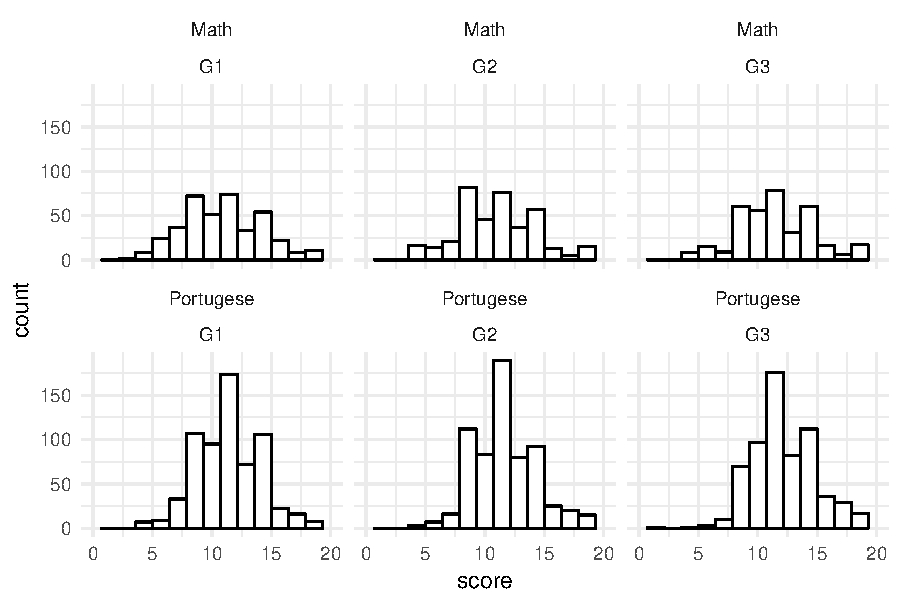
\includegraphics[width=1\linewidth]{studentAPA_comp_files/figure-latex/fig1-1} 

}

\caption{Distributions of class scores.}\label{fig:fig1}
\end{figure}

\begin{figure}

{\centering 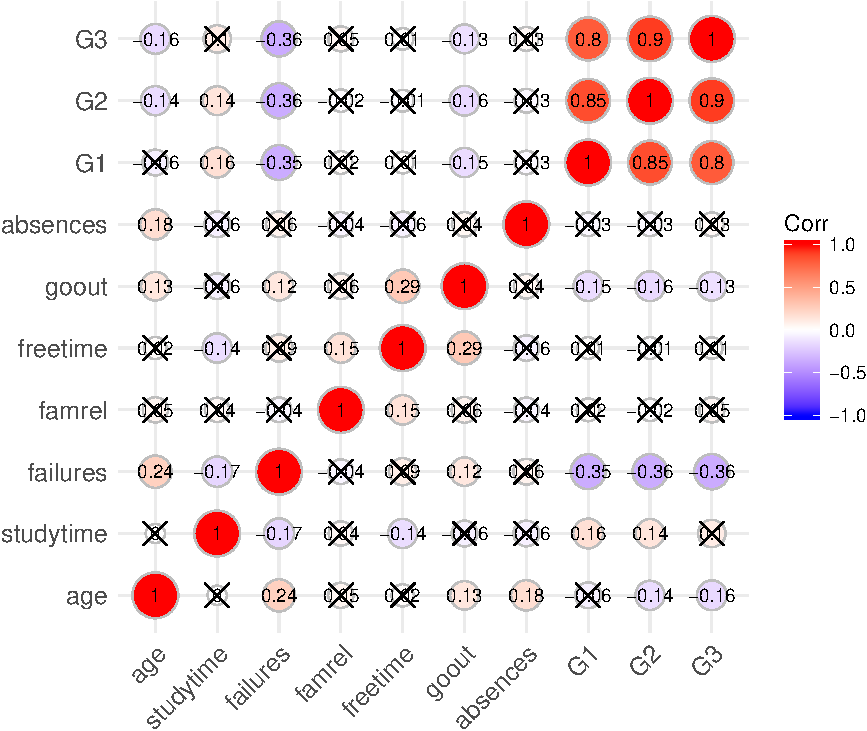
\includegraphics[width=0.7\linewidth]{studentAPA_comp_files/figure-latex/fig2-1} 

}

\caption{Correlations of numeric variables in the math data.}\label{fig:fig2}
\end{figure}

Descriptive statistics of grades separated by sex and school are
presented in Tables 1 and 2. Grades tended to increase over the course
of the semester. For example, the mean grade in the first Portugese exam
was 11.40 which increased to 11.91 by the last exam.

\begin{table}[tbp]
\begin{center}
\begin{threeparttable}
\caption{\label{tab:tbl1}Mean Portugese exam scores separated by sex and school}
\begin{tabular}{lllll}
\toprule
sex & \multicolumn{1}{c}{school} & \multicolumn{1}{c}{Exam 1} & \multicolumn{1}{c}{Exam 2} & \multicolumn{1}{c}{Exam 3}\\
\midrule
F & GP & 12.29 & 12.50 & 13.00\\
F & MS & 10.58 & 10.72 & 11.03\\
M & GP & 11.60 & 11.69 & 12.03\\
M & MS & 9.79 & 10.09 & 9.95\\
\bottomrule
\end{tabular}
\end{threeparttable}
\end{center}
\end{table}

\begin{table}[tbp]
\begin{center}
\begin{threeparttable}
\caption{\label{tab:tbl2}Mean Math exam scores separated by sex and school.}
\begin{tabular}{lllll}
\toprule
sex & \multicolumn{1}{c}{school} & \multicolumn{1}{c}{Exam 1} & \multicolumn{1}{c}{Exam 2} & \multicolumn{1}{c}{Exam 3}\\
\midrule
F & GP & 12.29 & 12.50 & 13.00\\
F & MS & 10.58 & 10.72 & 11.03\\
M & GP & 11.60 & 11.69 & 12.03\\
M & MS & 9.79 & 10.09 & 9.95\\
\bottomrule
\end{tabular}
\end{threeparttable}
\end{center}
\end{table}

Did men and women perform differently on the first exams in each class?
To test this, we conducted two separate two-sample t-tests on first exam
scores as a function of sex. The t-test on Portugese exam 1 was
significant \(\Delta M = -0.58\), 95\% CI \([0.16\), \(1.00]\),
\(t(589.90) = 2.69\), \(p = .007\), showing that women performed better
than men on the first Portugese exam,

The t-test on Math exam 1 was non-significant \(\Delta M = 0.61\), 95\%
CI \([-1.27\), \(0.05]\), \(t(383.79) = -1.82\), \(p = .069\), showing
no evidence for a difference between men and women on Math exam 1.

\begin{table}[tbp]
\begin{center}
\begin{threeparttable}
\caption{\label{tab:unnamed-chunk-1}ANOVA on period 1 Portugese scores.}
\begin{tabular}{lllllll}
\toprule
Effect & \multicolumn{1}{c}{$F$} & \multicolumn{1}{c}{$\mathit{df}_1$} & \multicolumn{1}{c}{$\mathit{df}_2$} & \multicolumn{1}{c}{$\mathrm{MSE}$} & \multicolumn{1}{c}{$p$} & \multicolumn{1}{c}{$\eta^2_G$}\\
\midrule
School & 70.78 & 1 & 644 & 6.62 & < .001 & .099\\
Sex & 13.25 & 1 & 644 & 6.62 & < .001 & .020\\
Guardian & 9.13 & 2 & 644 & 6.62 & < .001 & .028\\
\bottomrule
\end{tabular}
\end{threeparttable}
\end{center}
\end{table}

\section{Discussion}\label{discussion}

Understanding the relationship between language and math performance is
important for understanding learning. Our results are generally in line
with Abedi and Lord (2001) who found a relationship between language and
mathematics performance.

\section{References}\label{references}

\setlength{\parindent}{-0.5in} \setlength{\leftskip}{0.5in}
\setlength{\parskip}{8pt}

\hypertarget{refs}{}
\hypertarget{ref-abedi2001language}{}
Abedi, J., \& Lord, C. (2001). The language factor in mathematics tests.
\emph{Applied Measurement in Education}, \emph{14}(3), 219--234.

\hypertarget{ref-aust2015papaja}{}
Aust, F., \& Barth, M. (2015). \emph{Papaja: Create apa manuscripts with
rmarkdown}. Retrieved from \url{https://github.com/crsh/papaja}

\hypertarget{ref-collier1992synthesis}{}
Collier, V. P. (1992). A synthesis of studies examining long-term
language minority student data on academic achievement. \emph{Bilingual
Research Journal}, \emph{16}(1-2), 187--212.

\hypertarget{ref-horwitz1986foreign}{}
Horwitz, E. K., Horwitz, M. B., \& Cope, J. (1986). Foreign language
classroom anxiety. \emph{The Modern Language Journal}, \emph{70}(2),
125--132.

\hypertarget{ref-R}{}
R Core Team. (2016). \emph{R: A language and environment for statistical
computing}. Vienna, Austria: R Foundation for Statistical Computing.
Retrieved from \url{https://www.R-project.org/}






\end{document}
